\section{Introduction}

\begin{frame}
	\frametitle{The Importance of Hydrological Forecasting}
	\begin{block}{}
		Understanding hydrological processes has become increasingly critical in natural resource management. Suitable forecasting allows the anticipation capacity of extreme hydrological events such as droughts and heavy rainfall.
	\end{block}
	\begin{figure}
		\centering
		\begin{subfigure}[b]{0.45\textwidth}
			\centering
			\includegraphics[width=\textwidth, height=3.8cm]{figures/drought.jpg}
			\caption{Drought Condition}
		\end{subfigure}
		\hfill
		\begin{subfigure}[b]{0.45\textwidth}
			\centering
			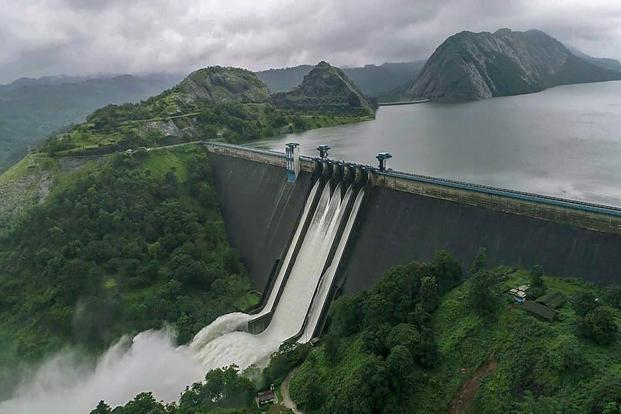
\includegraphics[width=\textwidth, height=3.8cm]{figures/full_dam.jpg}
			\caption{Full Dam}
		\end{subfigure}
	\end{figure}
	
	\begin{block}{\textcolor{myNewColorB}{\textbf{Challenges}}}
		Non-linearities, high stochasticity, and complex water resource patterns.
	\end{block}
	
\end{frame}